% Template for NIME 2023

% Modified by Adnan Marquez-Borbon 30 November 2022
% Modified by Courtney Reed 28 November 2022
% Modified by Joe Wright 14 December 2019
% Modified by Niccolò Granieri 10 October 2018 
% Modified by Angelo Fraietta 23 December 2018
% Modified by Angelo Fraietta 22 November 2018
% Modified by Rodrigo Schramm on 22 September 2018
% Modified by Luke Dahl on 17 October 2-17
% Modified by Cumhur Erkut on <2016-10-11 Tue>
% Modified by Edgar Berdahl on 5 November 2014
% Modified by Baptiste Caramiaux on 25 November 2013
% Modified by Kyogu Lee on 7 October 2012
% Modified by Georg Essl on 7 November 2011
%
% Based on "sig-alternate.tex" V1.9 April 2009
% This file should be compiled with "nime-alternate.cls"

% \documentclass{nime-alternate} % Uncomment when publishing final version
\documentclass{nime-alternate_MANUSCRIPT} % remove conference information

% Uncomment only one of the ones below
\usepackage{anonymize} 		   %Uncomment this line to publish
% \usepackage[blind]{anonymize}%Uncomment this line for blind review

% Package that enables the use of accents and non 
% standard characters
\usepackage[utf8]{inputenc}

\usepackage[implicit=false]{hyperref}

\begin{document}

% --- Author Metadata here ---
%\conferenceinfo{NIME'17,}{May 15-19, 2017, Aalborg University Copenhagen, Denmark.}
%\conferenceinfo{NIME'18,}{June 3-6, 2018, Blacksburg, Virginia, USA.}
%\conferenceinfo{NIME'19,}{June 3-6, 2019, Federal University of Rio Grande do Sul, ~~~~~~  Porto Alegre,  Brazil.}
% \conferenceinfo{NIME'20,}{July 21-25, 2020, Royal Birmingham Conservatoire, ~~~~~~~~~~~~ Birmingham City University, Birmingham, United Kingdom.}
%\conferenceinfo{NIME'22,}{June 28 - July 1, 2022, Waipapa Taumata Rau, T\={a}maki ~~~~~~~~ Makaurau, Aotearoa}

% \conferenceinfo{NIME'23,}{31 May–2 June, 2023, Mexico City, Mexico.}

\title{Delayed Gestural Control of Musical Sound \\
using \\
Online Unsupervised Temporal Segmentation}

% You need the command \numberofauthors to handle the 'placement
% and alignment' of the authors beneath the title.
%
% For aesthetic reasons, we recommend 'three authors at a time'
% i.e. three 'name/affiliation blocks' be placed beneath the title.
%
% NOTE: You are NOT restricted in how many 'rows' of
% "name/affiliations" may appear. We just ask that you restrict
% the number of 'columns' to three.
%
% Because of the available 'opening page real-estate'
% \label{key}% we ask you to refrain from putting more than six authors
% (two rows with three columns) beneath the article title.
% More than six makes the first-page appear very cluttered indeed.
%
% Use the \alignauthor commands to handle the names
% and affiliations for an 'aesthetic maximum' of six authors.
% Add names, affiliations, addresses for
% the seventh etc. author(s) as the argument for the
% \additionalauthors command.
% These 'additional authors' will be output/set for you
% without further effort on your part as the last section in
% the body of your article BEFORE References or any Appendices.

\numberofauthors{1} %  in this sample file, there are a *total*
% of EIGHT authors. SIX appear on the 'first-page' (for formatting
% reasons) and the remaining two appear in the \additionalauthors section.
%
\author{
% You can go ahead and credit any number of authors here,
% e.g. one 'row of three' or two rows (consisting of one row of three
% and a second row of one, two or three).
%
% The command \alignauthor (no curly braces needed) should
% precede each author name, affiliation/snail-mail address and
% e-mail address. Additionally, tag each line of
% affiliation/address with \affaddr, and tag the
% e-mail address with \email.
%
% 1st. author
\alignauthor
\anonymize{Juan Ignacio Mendoza}\\
       \affaddr{\anonymize{University of Jyväskylä, Finland}}\\ % Jyväskylä Jyvaskyla
%       \affaddr{\anonymize{University of Jyväskylä}}\\ % Jyväskylä Jyvaskyla
 %             \affaddr{\anonymize{University of Jyvaskyla}}\\ % Jyväskylä Jyvaskyla
%       \affaddr{\anonymize{Finland}}\\
%      \email{\anonymize{juigmend@student.jyu.fi}}
%% 2nd. author
%\alignauthor
%\anonymize{G.K.M. Tobin}\titlenote{\anonymize{The secretary disavows
%any knowledge of this author's actions.}}\\
%       \affaddr{\anonymize{Institute for Clarity in Documentation}}\\
%       \affaddr{\anonymize{P.O. Box 1212}}\\
%       \affaddr{\anonymize{Dublin, Ohio 43017-6221}}\\
%       \email{\anonymize{webmaster@marysville-ohio.com}}
%% 3rd. author
%\alignauthor \anonymize{Lars Th{\o}rv{\"a}ld}\titlenote{This author is the
%one who did all the really hard work.}\\
%       \affaddr{\anonymize{The Th{\o}rv{\"a}ld Group}}\\
%       \affaddr{\anonymize{1 Th{\o}rv{\"a}ld Circle}}\\
%       \affaddr{\anonymize{Hekla, Iceland}}\\
%       \email{l\anonymize{arst@affiliation.org}}
%\and  % use '\and' if you need 'another row' of author names
%% 4th. author
%\alignauthor \anonymize{Lawrence P. Leipuner}\\
%       \affaddr{\anonymize{Brookhaven Laboratories}}\\
%       \affaddr{\anonymize{Brookhaven National Lab}}\\
%       \affaddr{\anonymize{P.O. Box 5000}}\\
%       \email{\anonymize{lleipuner@researchlabs.org}}
%% 5th. author
%\alignauthor \anonymize{Sean Fogarty}\\
%       \affaddr{\anonymize{NASA Ames Research Center}}\\
%       \affaddr{\anonymize{Moffett Field}}\\
%       \affaddr{\anonymize{California 94035}}\\
%       \email{\anonymize{fogartys@amesres.org}}
%% 6th. author
%\alignauthor \anonymize{Anon Nymous}\\
%       \affaddr{\anonymize{Redacted }}\\
%       \affaddr{\anonymize{8600 Datapoint Drive}}\\
%       \affaddr{\anonymize{San Antonio, Texas 78229}}\\
%       \email{\anonymize{cpalmer@prl.com}}
}
% There's nothing stopping you putting the seventh, eighth, etc.
% author on the opening page (as the 'third row') but we ask,
% for aesthetic reasons that you place these 'additional authors'
% in the \additional authors block, viz.
%\additionalauthors{Additional authors: \anonymize{John Smith (The Th{\o}rv{\"a}ld Group,}
%email: {\texttt{\anonymize{jsmith@affiliation.org}}}) and \anonymize{Julius P.~Kumquat 
%(K. Consortium,} email: {\texttt{\anonymize{jpkumquat@consortium.net}}}).}
%\date{30 July 1999}
% Just remember to make sure that the TOTAL number of authors
% is the number that will appear on the first page PLUS the
% number that will appear in the \additionalauthors section.

% For your initial submission you MUST ANONYMIZE the authors.

\maketitle

\begin{abstract}
The recognition of continuous gestures for control of electronic musical systems by means of machine learning has two notable constraints. The first is that the system needs to be trained with individual example gestures, the starting and ending points of which need to be well defined. The second constraint is time required for the system to recognise that a gesture has occurred, which may prevent the quick action that musical performance typically requires. This article describes a method for real-time unsupervised segmentation of gestures. This method allows a user to continually perform without explicitly indicating the starting and ending of gestures in order to train the machine learning algorithm. Furthermore, an apparatus for control of musical sound was devised to demonstrate the feasibility of the segmentation method, incorporating the time required by the process into the interaction paradigm. The real-time unsupervised automatic segmentation method and the concept of delayed control may be exploited in the design and implementation of systems that facilitate seamless human-machine musical interaction without the need for quick response time, for example when using broad motion of the human body.
\end{abstract} 

%\vspace{0.35cm}	

\keywords{unsupervised, segmentation, machine learning, gesture, recognition, accelerometry, music, controller, interface, DMI}

% ------- CCS Concepts
% Here is where you enter the CCS Concepts for your paper.
%
% It is strongly recommended that authors view the submission form
% prior to starting to write the paper, which includes information 
% on the CCS Concepts. 
% 
% The 2012 ACM Computing Classification System (CCS) replaces the
% traditional 1998 version, which has served as the de facto 
% standard classification system for the computing field. It is
% being integrated into the search capabilities and visual topic 
% displays of the ACM Digital Library. Please enter the CCS XML code 
% for the classification terms that describe your paper. To get the 
% XML code, please use the following procedure, which is
% demonstrated using three NIME-related example terms: Applied
% computing~Sound and music computing, Applied computing~Performing
% arts, and Information systems~Music retrieval.
%
% 1) Browse to the website http://dl.acm.org/ccs_flat.cfm.
% 2) Select one to three classification terms from the website that
%    describe your paper (e.g. for the example paper Applied
%    computing~Sound and music computing, Applied 
%    computing~Performing arts, and Information systems~Music
%    retrieval.).
% 3) For each classification you need to select the relevance
%    (e.g. for this example, Sound and music computing is "high",
%    Performing arts is "low", and Music retrieval is "Medium")
% 4) Once you have selected the last term, click on "view CCS Tex
%    Code". This will generate some code, which includes some CCSXML
%    and some lines beginning with \ccsdesc.
% 5) Keep all of this code, as you will need it for entering into
%    the Precision Conference System paper submission form.
% 6) For this document, keep only the \ccsdesc lines. Here is what
%    you would paste for the classification example:

\ccsdesc[500]{Human~centered computing}
\ccsdesc[500]{Computing methodologies~Machine learning}
%\ccsdesc[300]{Applied computing~Sound and music computing}
\ccsdesc[100]{Information systems~Music retrieval}
\ccsdesc[100]{Applied computing~Performing arts}

% this line creates the CCS Concepts section.
\printccsdesc

\vspace{0.35cm}	

\section{Introduction}

Musical instruments are usually designed to be controlled with fine movements of hands and fingers, as they afford precision and speed. These qualities are often described as the foundations of responsiveness, believed to be indispensable for musical expression. The instrument thus becomes an extension of the human body. These ideas have permeated into the design of digital musical instruments (DMI) \cite{Moore_1988}, and a response time approaching zero has become a standard goal \cite{Wessel_Wright_2002, Jack_etal_2018, McPherson_etal_2016}.

\vfill\eject

Similar aspirations have been present when designing DMI that are made to recognise gestures ``in the air", using machine learning techniques. For example, a musician wears, holds or stands in front of, a device that may sense position (i.e., static gestures) or motion (i.e., continuous gestures). The musician makes a gesture in free space, for example describes a circle with the head, or wiggles a hand, or stands in a particular pose. The DMI would learn these gestures in a process called ``training". Then, the DMI would recognise the learned gestures when they are performed. The recognition of a gesture can be mapped to a musical action, such as triggering a sound, activating an effect, etc. (e.g., \cite{Gillian_2011}).

Two algorithms and variations of them have been extensively used to recognise continuous gestures, regardless of the sensing technology: Dynamic Time Warping (DTW) \cite{Gillian_etal_2011} and Hidden Markov Models (HMM) \cite{Bevilacqua_etal_2010}. Both can estimate the likelihood that a gesture being performed corresponds to a gesture that has been learned in the training stage. However, this likelihood may change while the gesture is being executed, therefore it is only possible to reliably confirm the recognised gesture after it has reached its end. 
This adds time to the recognition, arguably reducing responsiveness. In addition, these algorithms need to be trained with individual gestures, which requires the beginning and ending of gestures to be explicit.

Given a stream of data from a sensor, individual gestures may be extracted by a process called ``segmentation". This may be accomplished by a procedure that dictates the start and ending points of gestures. For example, when training the algorithm the user presses a button (e.g., \cite{Merril_Paradiso_2005}) or makes pauses between gestures (e.g., \cite{Murad_etal_2017}). While this constraint has not prevented the use of the algorithms mentioned above in new interfaces for musical expression, the ability of a machine to recognise and learn gestures without explicit training would open new avenues for human-machine musical interaction. Furthermore, the time required for the recognition of continuous gestures might not be a disadvantage if when designing a DMI we don't hold the same standards of responsiveness as for the human voice or other non-electronic instruments. Consider that digital technologies have greatly expanded our possibilities for control of sound, far beyond what is possible with the human voice or with non-electronic devices. Why should we hold ourselves from exploring forms of gestural control that are not quick and precise, but instead slow and imprecise such as broad motion of the human body?
	
This article describes a system that was devised as a proof of concept towards exploring the feasibility of unsupervised learning of patterns in a continuous input signal, in a musical application that doesn't require quick responsiveness. The system is conceptually a musical instrument in a broad sense, for it essentially allows a user to control sound.

One key quality of this instrument and the innovation presented here, is that it segments gestures without the need of explicitly indicating their starting and ending points. These gestures may trigger actions that control sound. However, the detection of gestures needs some time to occur. It might be just a fraction of a second, but it is enough to be perceived as not instantaneous. This would normally be considered a disadvantage, but in the context of this study it is not. Furthermore, the capability of detecting gestures without explicit training is proposed as a resource to design musical instruments that may seamlessly interact with their users, acting more as agents than as tools. The next section presents a description of the algorithm that segments gestures without explicit indication, a process called unsupervised temporal segmentation. Then the development of the proof-of-concept instrument is described, followed by a discussion with suggestions for further research.

\begin{figure}[t!]
	\centering
		%\includegraphics[trim={1cm 1.4cm 1cm 5.6cm}, clip=true, width=1\columnwidth]{fig_1}
		%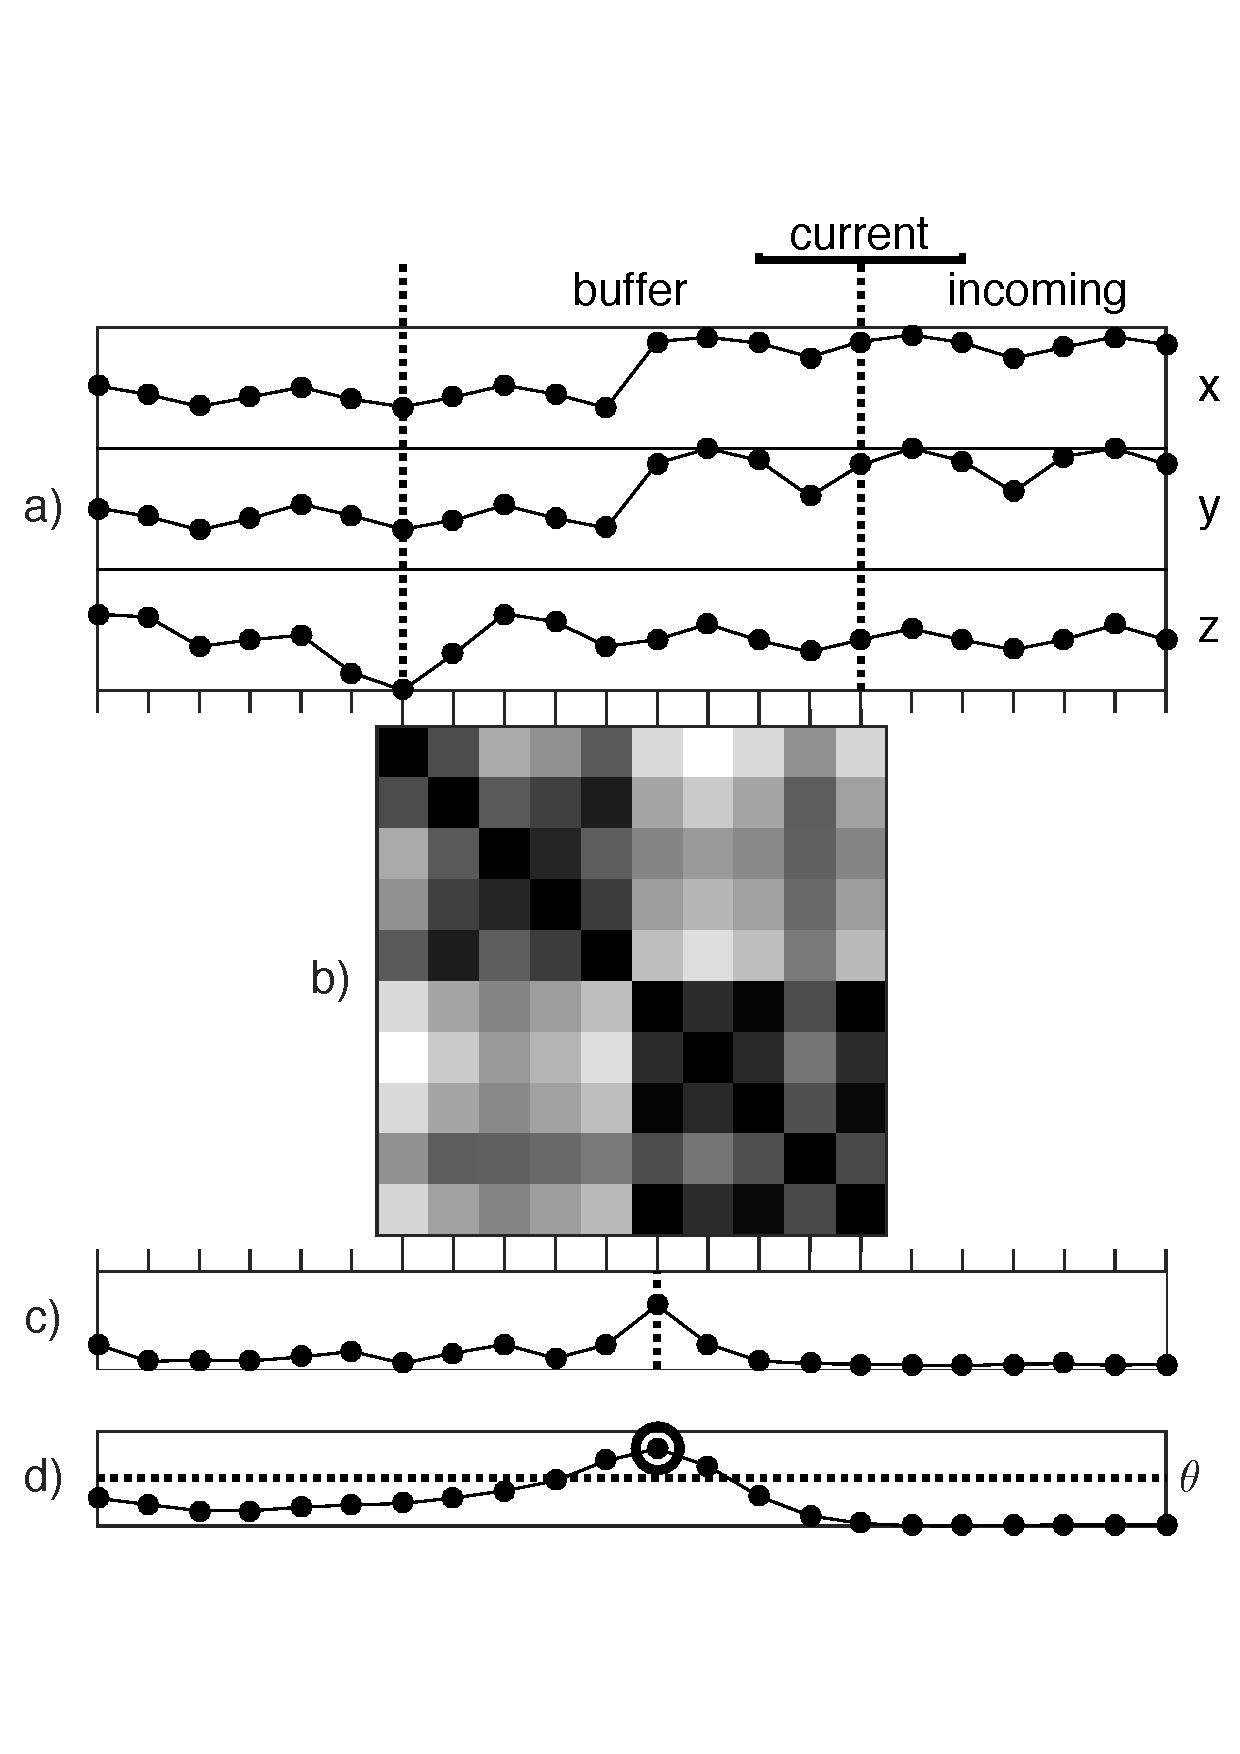
\includegraphics[trim={0.3cm 3.5cm 0.3cm 3.5cm}, clip=true, width=1\columnwidth]{fig_1_LO}
		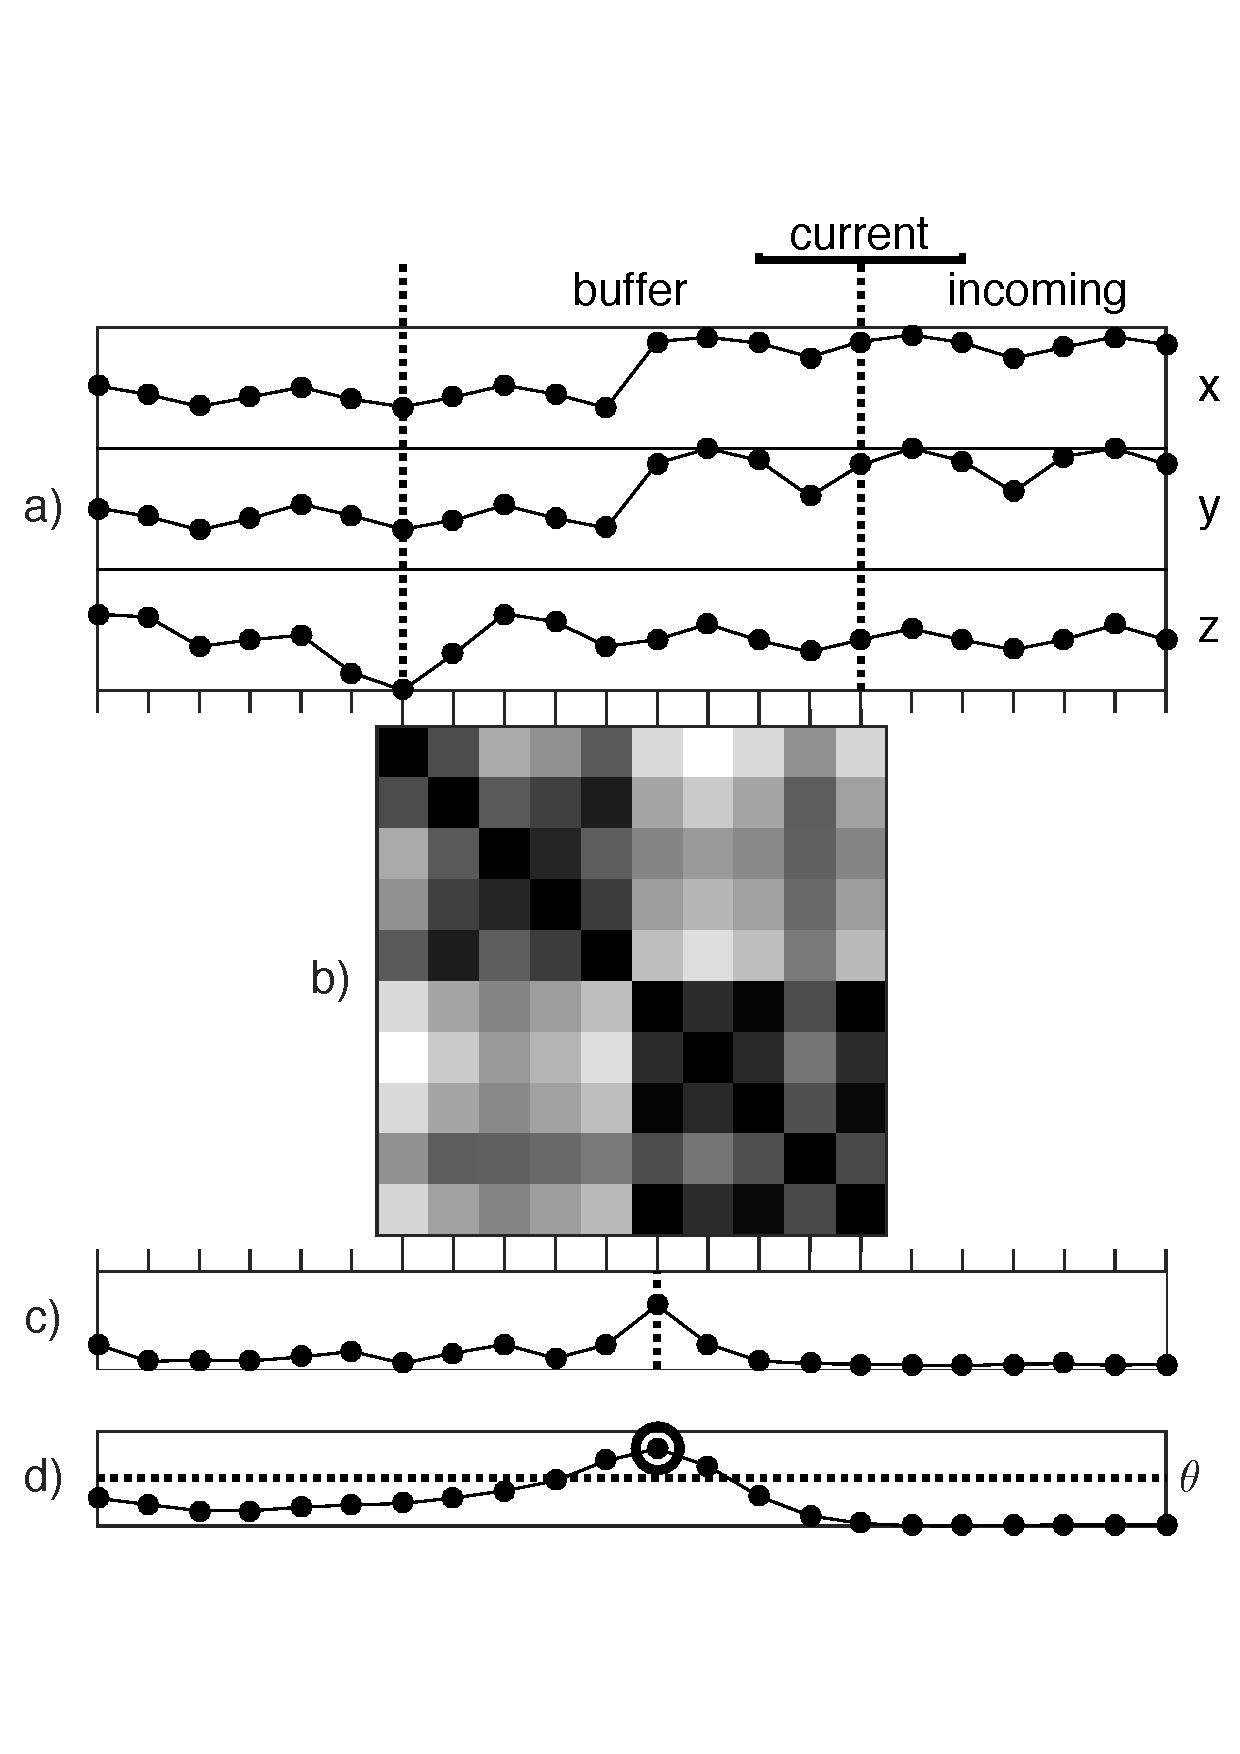
\includegraphics[trim={0.3cm 3.5cm 0.3cm 3.5cm}, clip=true, width=0.9\columnwidth]{fig_1_LO}
	\caption{Online temporal segmentation. Horizontal axes represent time. (a) is triaxial accelerometer data. (b) is self-similarity matrix $D$ of data in the buffer  $W_{nov}$, where lighter shades represent more distance. (c) is novelty score $N$, where the vertical dotted line indicates the current result. (d) is the smoothed novelty score $N'$, where $\theta$ is a threshold and the point in a circle is the selected peak indicating a  boundary. Note that this visualisation shows $N$ and $N'$ aligned in time, but in practice there will be a lag due to the filter and the test for a peak.}
	\label{fig_1}
%\vspace{0.5cm}	
\end{figure}

\section{Online Unsupervised Temporal Segmentation}\label{OUTS}

A signal may be segmented using the algorithm described by Foote \cite{Foote_2000}. That algorithm has seen application in segmentation of musical audio and video \cite{Foote_Cooper_2003, Tardieu_etal_2009}. Also, it has been tested for segmentation of dancing motion captured by an accelerometer \cite{Mendoza_Thompson_2017} and daily activity recorded by wearable devices equipped with accelerometers \cite{Mendoza_etal_2022, Rodrigues_Probst_Gamboa_2021}. The parameters of the algorithm can be adjusted to detect boundaries of segments (also known as change-points) at different timescales. The cited sources had described the use of the algorithm on recorded data. Conversely, Schätti \cite{Schatti_2007} described an online version of the algorithm which detects boundaries of audio data while the data is being produced. Later,  
% \anonymize{foooooooooooooooooo}
Mendoza \cite{Mendoza_2022} 
reported perceptual tests of the algorithm applied to segmentation of dancing motion captured by a hand-held device containing an accelerometer. In that study the algorithm's segmentation was compared to manual segmentation of video recordings of the dancing. The algorithm's meta-parameters needed to be optimised for each accelerometry recording. Further analyses revealed that the music used for the dance and the person doing the manual segmentation were the main factors affecting the quality of the computed segmentation. These results suggest that the algorithm is suitable for gestural control, albeit the algorithm's meta-parameters might need contextual adjustment. While the interested reader may consult the cited sources for detailed descriptions, below a brief description is provided of the implementation of the online segmentation algorithm for the system described in this article. It uses the same principle of buffering and computation of a local distance matrix, as described by Schätti \cite{Schatti_2007} and 
% \anonymize{foooooooooooooooooo}
Mendoza \cite{Mendoza_2022}.

Firstly, a two-dimension kernel $K$ is produced by the Kronecker product of a checkerboard matrix and an only-ones matrix of width $n$. Then $K$ is tapered by multiplying it element-wise with a two-dimensional Gaussian. For convenience, $K$ is computed only once and stored in memory. The input to the real-time segmentation algorithm is a stream $M$ of triaxial accelerometry data points, herein referred to as “frames” $F=(f_x,f_y,f_z )$ sampled at regular intervals. A window of $n$ frames is stored in a buffer $W_{nov}$ (Figure~\ref{fig_1}a). For each incoming frame the last frame in the buffer is removed while the current frame is stacked in the first position, and distance matrix $D \in \mathbb{R}^{n \times n}$  is computed for $W_{nov}$ (Figure~\ref{fig_1}b). For this study Euclidean and City Block distances were tested with no practical difference, although the latter was preferred because it is computationally faster as it doesn't compute the square root. At the arrival of each data frame $F$, the inner product between $K$ and $D$ is computed, resulting in a new point in novelty score $N$ (Figure~\ref{fig_1}c). 

Distance matrix $D$ is symmetric, therefore only one of its triangles over or under the diagonal is relevant and it may be represented as a vector. Matrix $D$ is initialised with allocation values (e.g., zeros). As data frames arrive, the  distance between the current frame and all the other frames in the buffer is computed. At the arrival of each new frame, the inner product of the upper or lower triangle of $D$ and the corresponding triangle of $K$ is computed resulting in a novelty value. After this is done and before computing the next novelty value, the values within $D$ are shifted, discarding the distances between the oldest frame and the newer ones.

Then, a low-pass filter is applied to $N$ by convolving it with a Gaussian window of length $n_{filt}$, resulting in a smooth novelty score $N'$. If the current novelty score value is a peak over a threshold $\theta$, it is deemed to be a segmentation boundary (Figure~\ref{fig_1}d). The relevance of segmentation boundaries may be adjusted with parameter $\theta$ (e.g., to prevent segmentation of noise) while the timescale of the segments is adjusted with parameter $n$. In the implementation described here, $N'$ is rescaled to $\{0,1\}$ when a new maximum occurs, and $\theta$ is a factor. The novelty peak is located at the center of the kernel and the filter window, and the test for a peak requires only three frames. Therefore, the lag (i.e., frames needed to carry out the computation) for the whole procedure is $(n+ n_{filt})/2+3$ frames.

\section{Proof of Concept}

\subsection{Hardware}

A polystyrene ball having 12 cm. of diameter was cut in half and the interior was carved to fit a Myo armband controller (Figure~\ref{fig_2}). The Myo was originally designed by Thalmic Labs to be worn on the forearm. It has electromyographic sensors to detect muscle contraction, a triaxial accelerometer, a triaxial gyroscope, and a magnetometer measuring on the horizontal plane when the armband is worn on the forearm in horizontal position. The two halves of the ball are put together restoring the spherical shape, but it can be easily disassembled to recharge the battery of the Myo. The data from the sensors is broadcast in real time using the Bluetooth Low-Energy (BLE) specification. The BLE signal is captured by a personal computer nearby, and a piece of software by Rodrigo Schramm\footnote{See~\cite{Visi_2017}.~Software~available:~\href{https://github.com/federicoVisi/KineToolbox/blob/master/input\%2BML/DaemonMYO}{https://github.com/federicoVi\\si/KineToolbox/blob/master/input\%2BML/DaemonMYO}} outputs the data in Open Sound Control (OSC) format to a User Datagram Protocol (UDP) port, where it can be accessed by other software as described below. This controller was used for its convenience, as it was available to the researcher along with the software to access the data in real time. Only the triaxial accelerometer signal is used by the system described in this article.

\begin{figure}[t!]
   \setlength\tabcolsep{2pt} 
    \begin{tabular}{cc}
        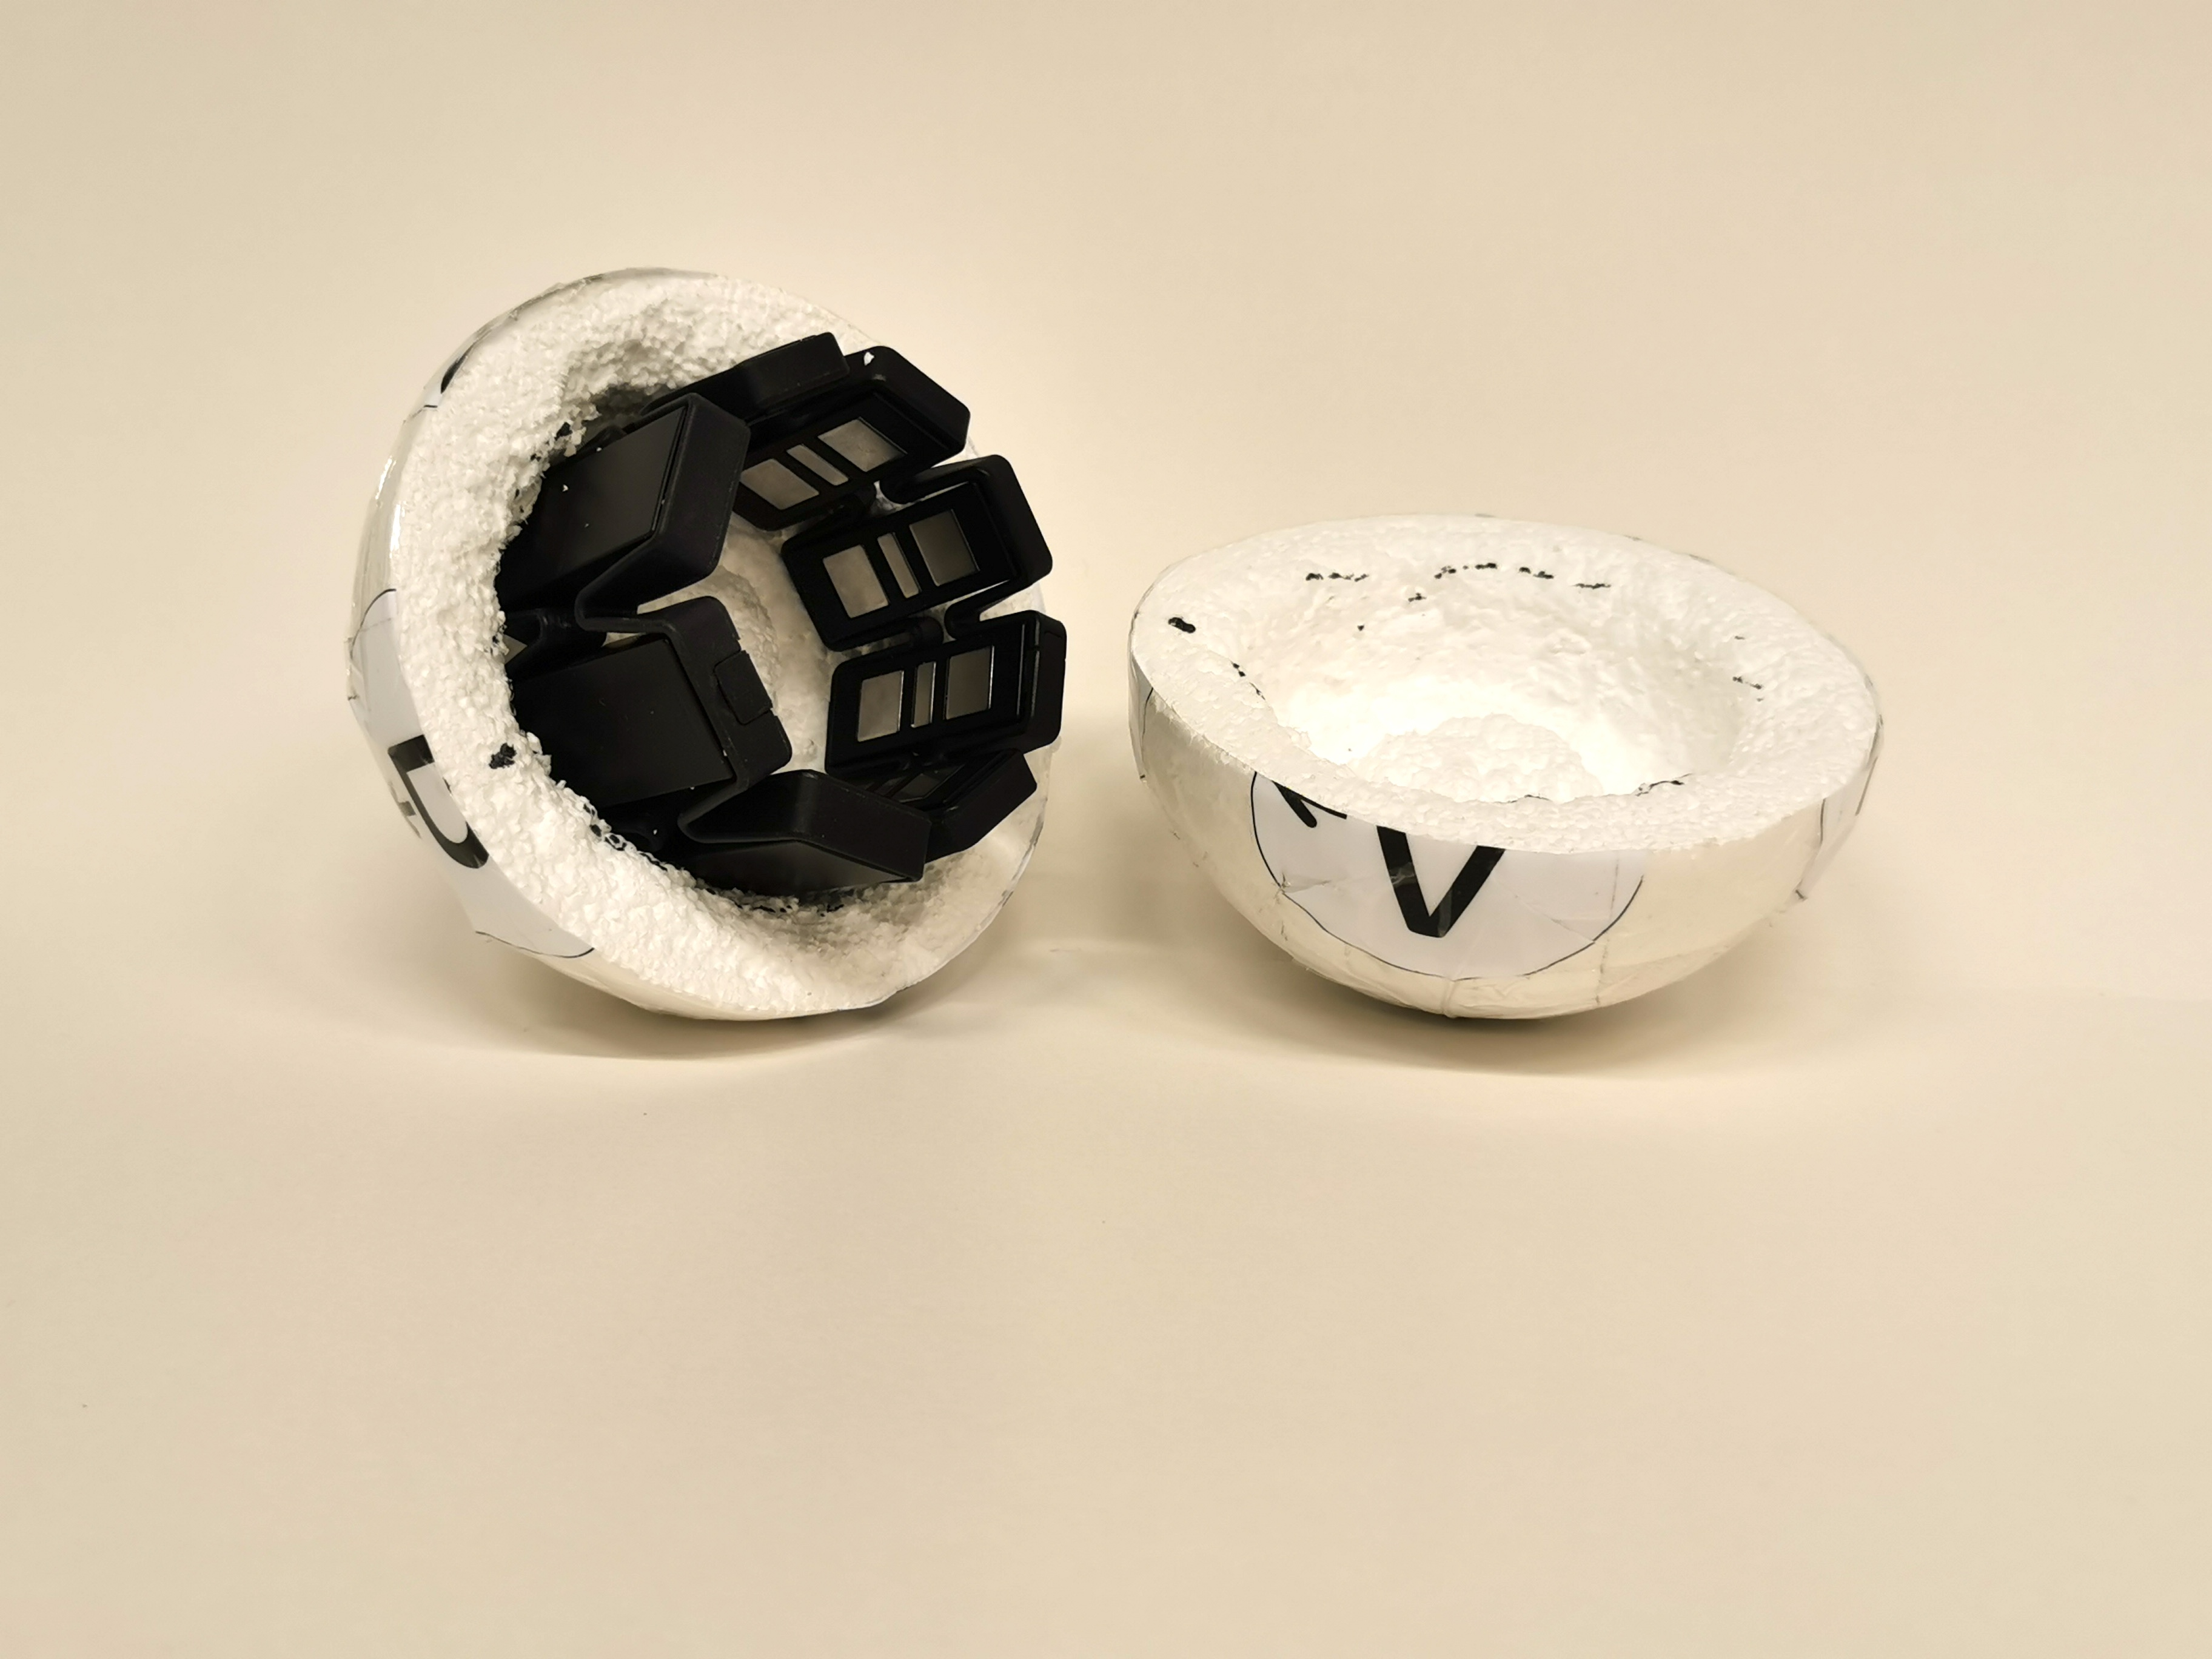
\includegraphics[trim={10cm 24cm 10cm 6cm}, clip=true, width=0.48\columnwidth]{ball_open}
        &
        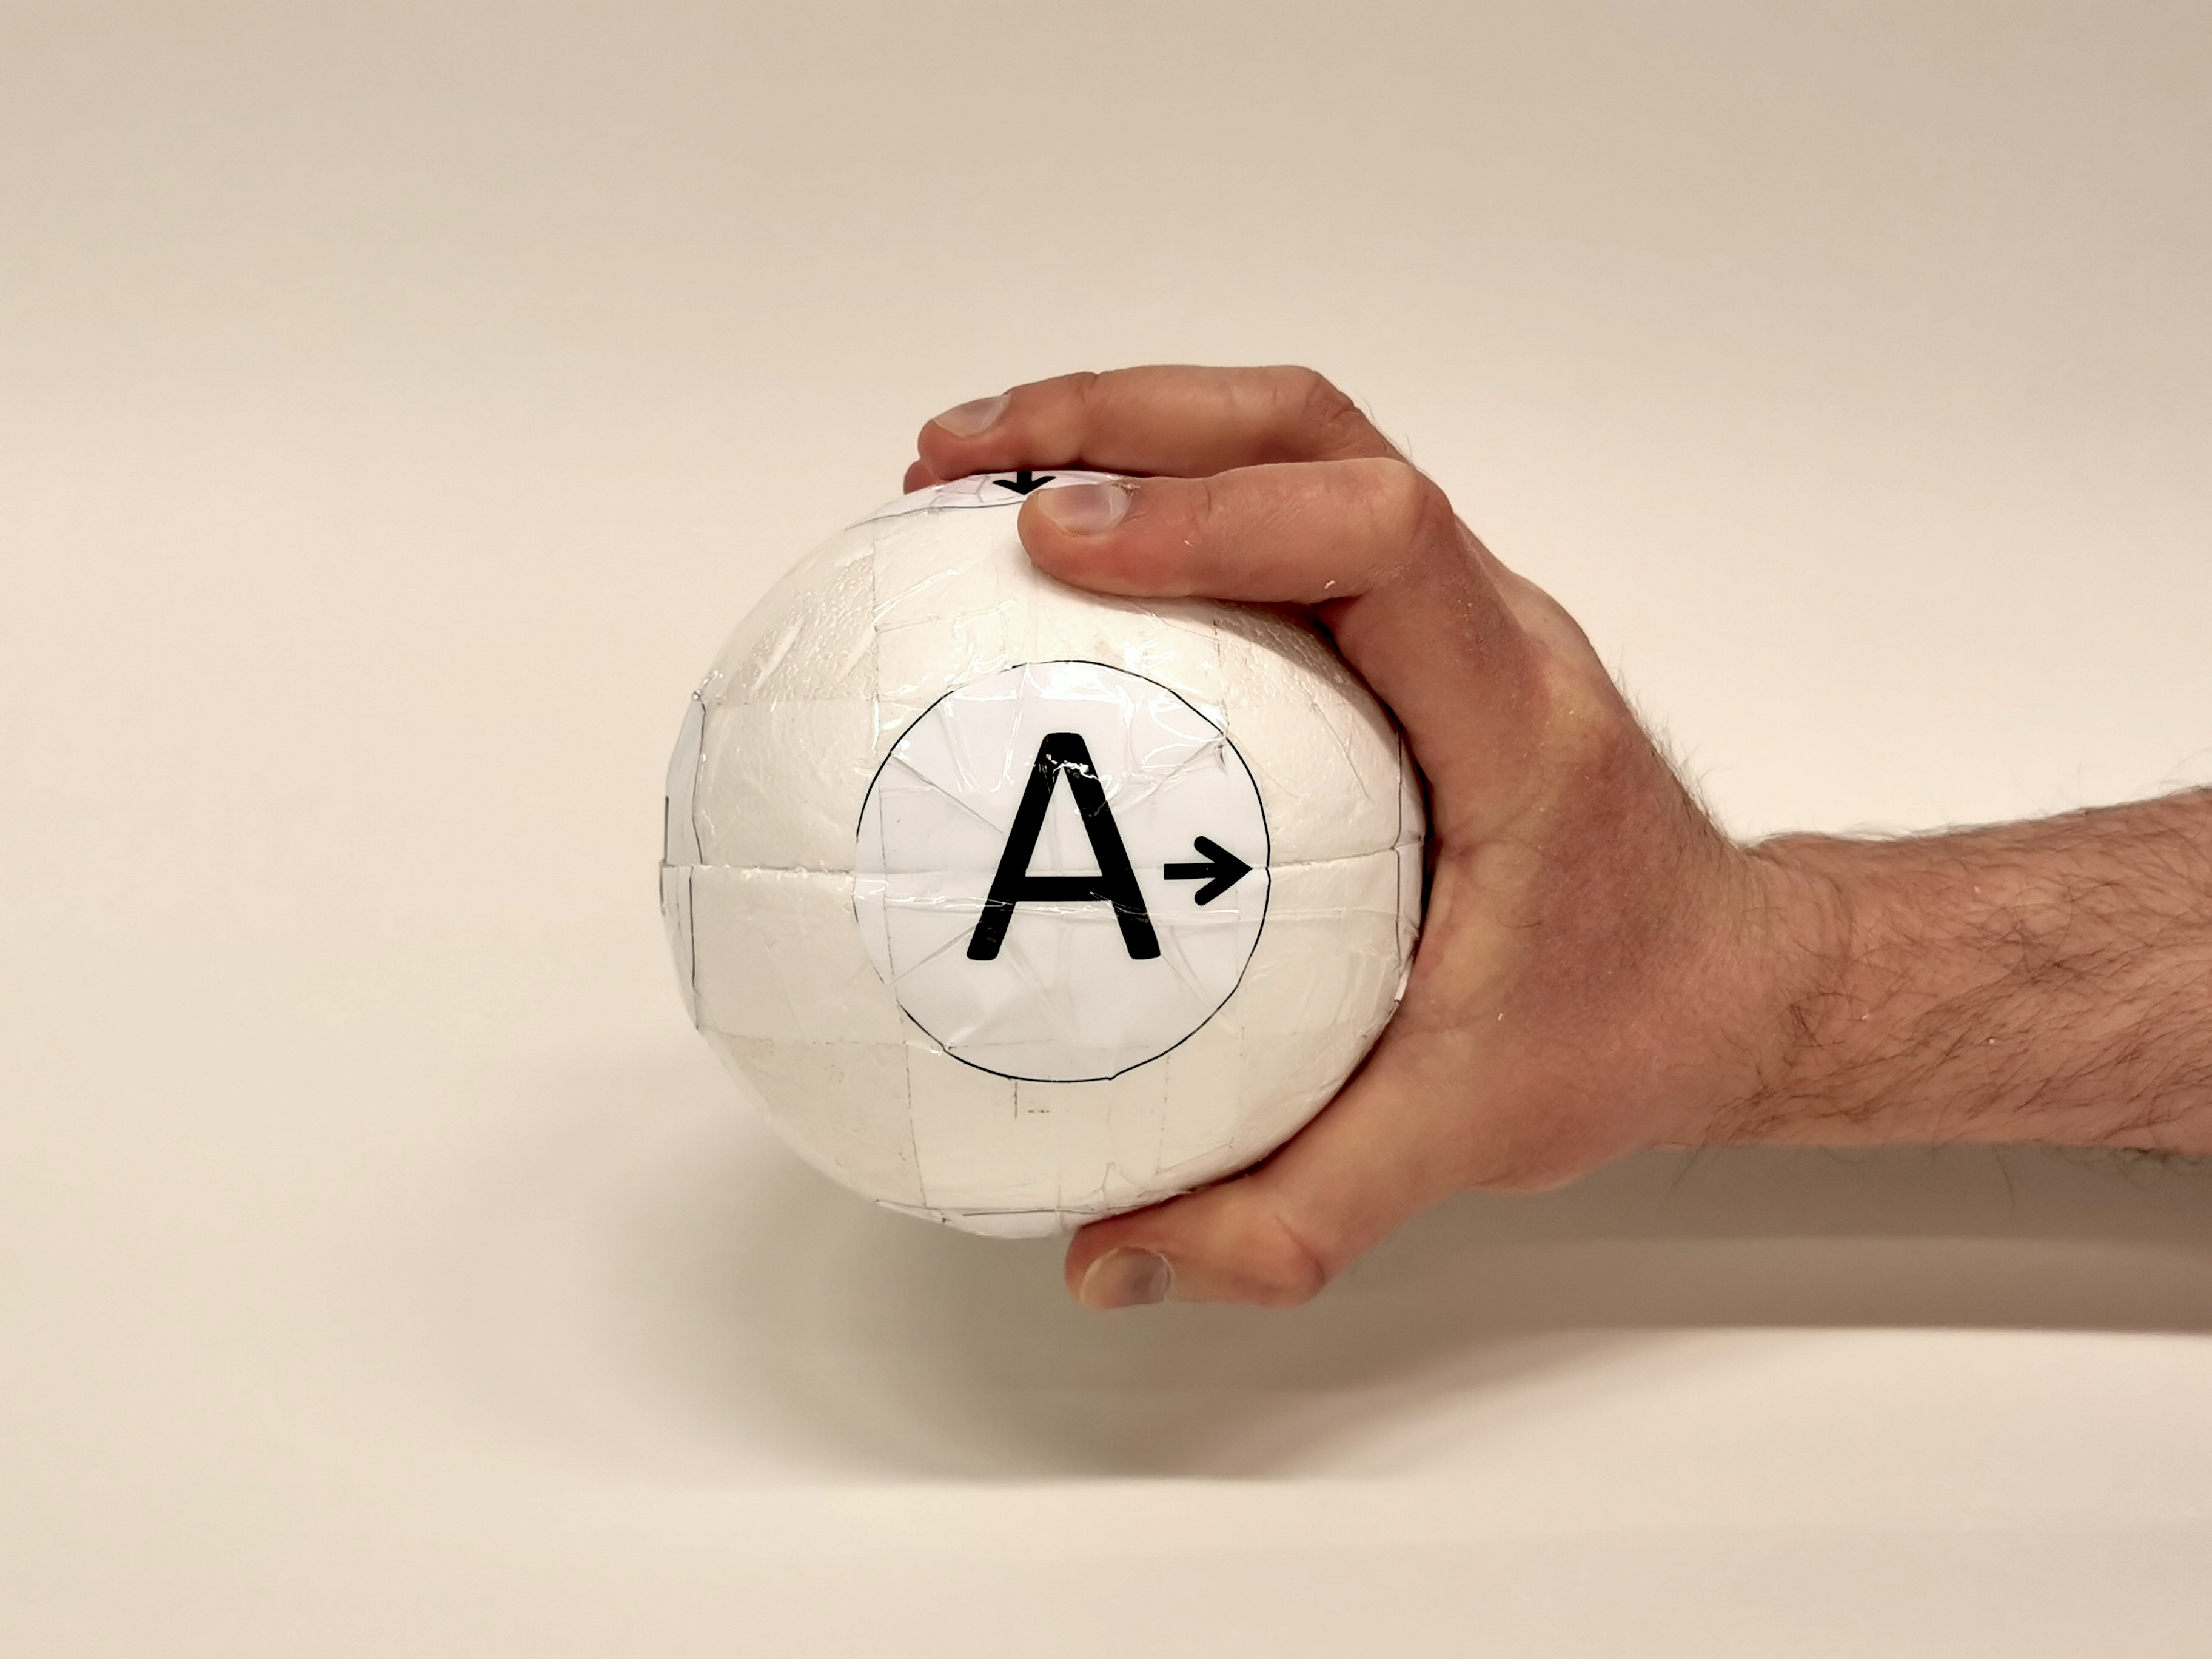
\includegraphics[trim={20cm 15cm 0cm 15cm}, clip=true, width=0.48\columnwidth]{ball_handheld}
    \end{tabular}
	\caption{Left -- Carved open polystyrene ball with the Myo armband in it. Right -- Closed ball.}
	\label{fig_2}
\vspace{0.6cm}
\end{figure}

\subsection{Software}

The segmentation procedure described in section \ref{OUTS} can detect boundaries between motion patterns performed with the hand-held controller continuously. This implies that the patterns may be gestures executed without the need to indicate their start or end. Segmentation occurs in real time, and the result (a gesture boundary) is obtained with a delay time comprising the lag of the procedure as described in section \ref{OUTS}, plus computation time. Given these properties, the segmentation process was deemed to be useful as a preprocessing stage to map data from a controller to sound, instead of directly mapping raw sensor data. However, because of the delay in the result, any action connected to the detection of a boundary cannot be performed immediately. Also, a further meta-parameter was incorporated to prevent segments of less than a given length $n_{min}$. This parameter was incorporated because the transitions between gestures may be detected by the system as short segments. The segmentation procedure was implemented in the Pure Data programming environment, which receives the accelerometry data using OSC as described in the previous subsection. Also the musical application and its graphical user interface were implemented in Pure Data, as described below. The software is free and available (see Appendix).  

The detected segments, each comprising a full gesture, are stored in memory and fed to a machine-learning process, so that later they can be recognized when performed continuously. The DTW algorithm was used for gesture learning and recognition. This algorithm was chosen as it is available in the easy-to-use software Wekinator \cite{Fiebrink_etal_2009, Wekinator_website}, which communicates with Pure Data using OSC over a UDP port. However, another online learning and recognition algorithm could be used (e.g., HMM). As with segmentation, the result of the recognition has lag due to buffering and latency due to logical processing.

The segmentation and machine-learning processes are incorporated into a musical system that allows the user to reorder sections of an audio file. The sections are indicated by the segments detected in the hand-held controller’s signal. The use of the system comprises two main stages: Cut and Perform. In the Cut stage (Figure~\ref{fig_3}) the system plays the audio file in its entirety while the user performs distinct gestures. The boundaries between these gestures are detected in real time by the segmentation process and their time location is stored and labelled with a sequential index (i.e., 1, 2, 3,…). As this happens, the segments of the triaxial accelerometry signal are also fed as individual examples to the gesture learning process (i.e., “one-shot” learning) and stored for later recognition. Also, a green vertical line is placed in the graphical user interface over a plot of the signal, to indicate that the gesture has been successfully segmented (Figure~\ref{fig_5}).

After the Cut stage the Perform stage can be executed. In the Perform stage (Figure~\ref{fig_4}) the gesture recognition process is continuously comparing the incoming triaxial accelerometry signal, to all the segments that were stored when executing the Cut stage. The segment that is closest to a stored segment will be deemed a match and its corresponding audio section will be played in a loop. The recognition process will continue to assess the similarity between the incoming signal and the stored segments. If a gesture different than the current is recognised, then the corresponding audio section will be played once the current audio section reaches its end. 

\begin{figure}[t!]
	\centering
		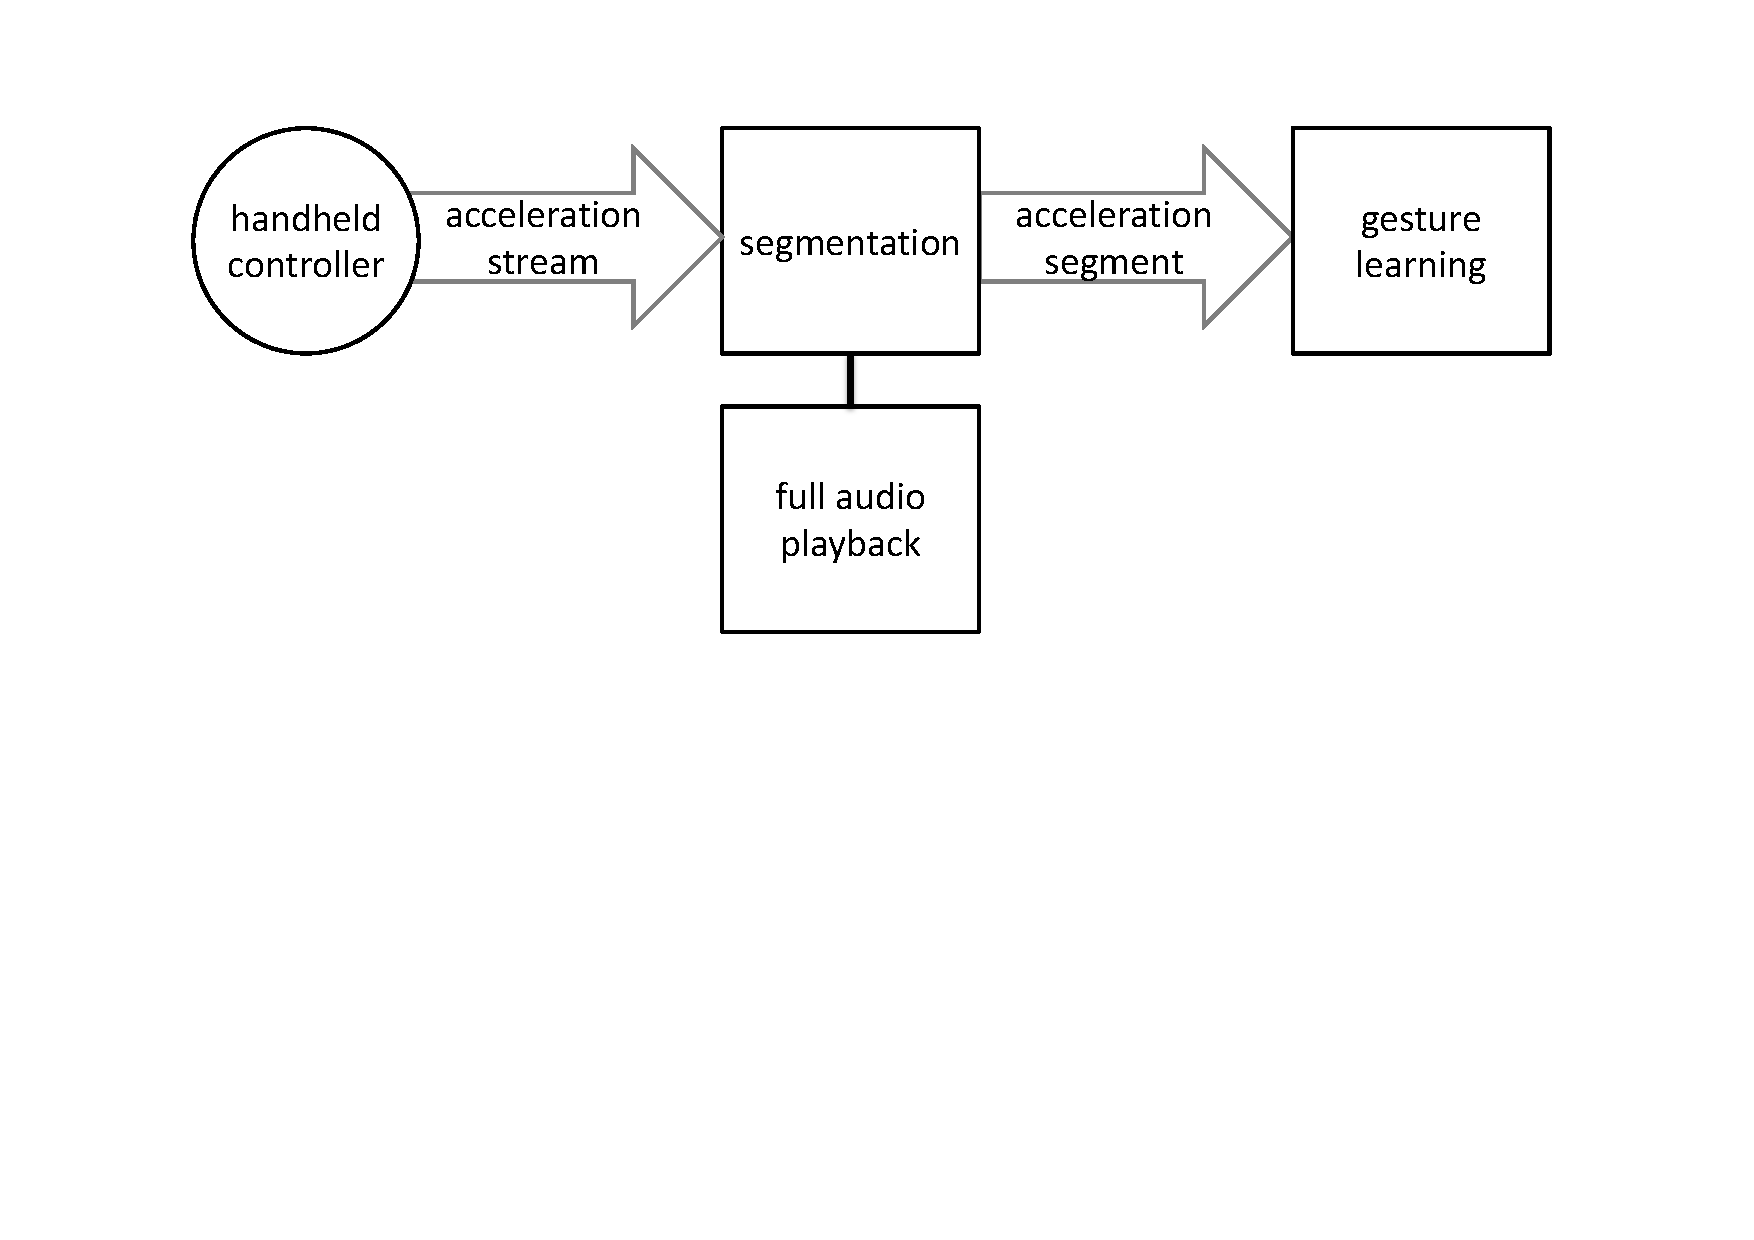
\includegraphics[trim={3.2cm 10.2cm 3.2cm 2.1cm}, clip=true, width=1\columnwidth]{cut}
	\caption{Cut -- The triaxial acceleration stream is segmented while the audio file plays.}
	\label{fig_3}
\end{figure}

\begin{figure}[t!]
%\vspace{0.6cm}
\vspace{1cm}
	\centering
		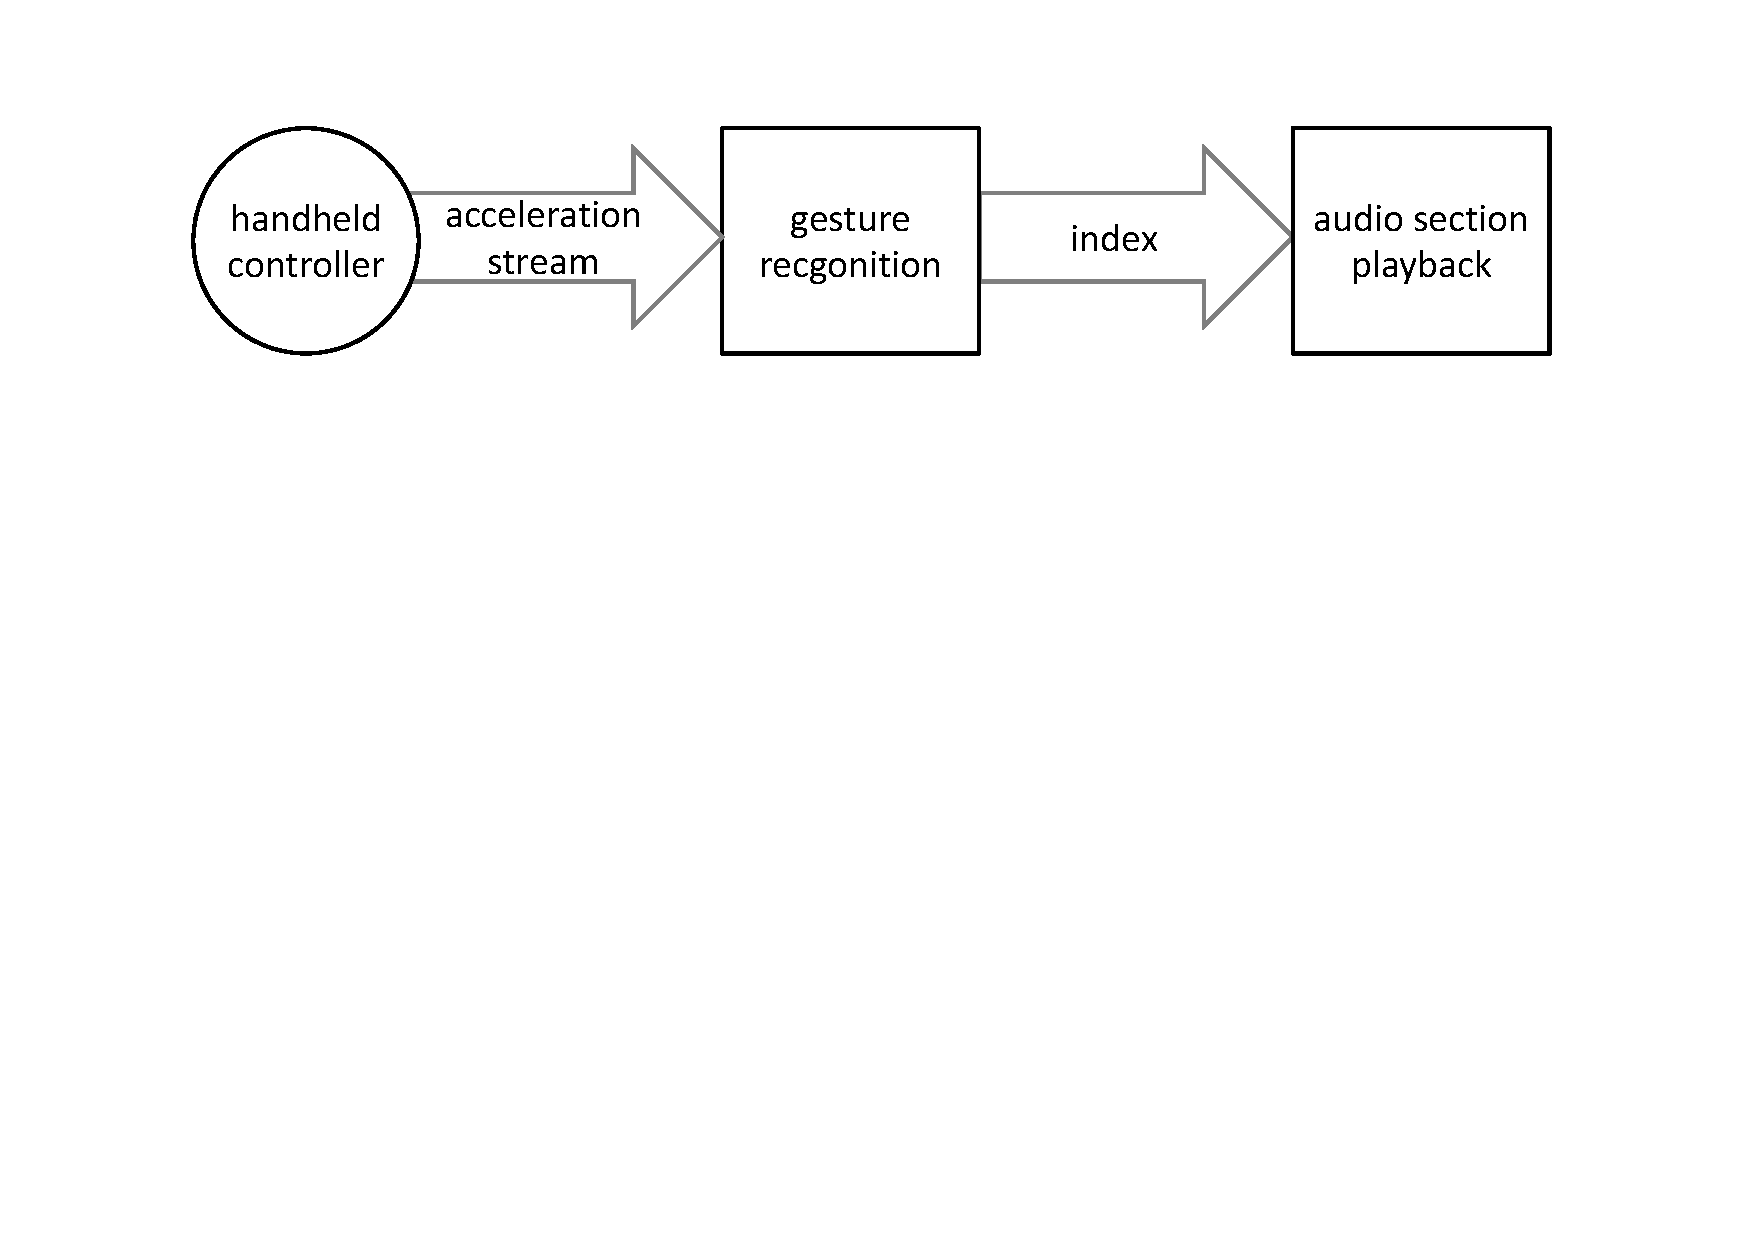
\includegraphics[trim={3.2cm 14.9cm 3.2cm 2.1cm}, clip=true, width=1\columnwidth]{perform}
	\caption{Perform -- Gestures recognised in the triaxial acceleration stream indicate the next audio segment to play.}
	\label{fig_4}
\end{figure}

\subsection{Testing}\label{Testing}

Testing, in the context of this study, refers to the assessment of the system’s components (Figures \ref{fig_3} and ~\ref{fig_4}) separately and progressively combined. This was done along the development process to inform the system’s design and implementation. One outcome of testing that is particular to the interaction paradigm presented here, is the discovery of gestures that work well with the system. This means gestures (whether they involve motion or not) and combinations of gestures that can be segmented, learned and recognised by the system. This involved the adjustment and fine-tuning of the system’s meta-parameters: timescale ($n$), upper bound threshold ($n_{min}$), novelty smoothing ($n_{filt}$), and novelty threshold ($\theta$). Also, parameters of the DTW process had to be adjusted but those are not discussed as the DTW algorithm is well known and documented \cite{Gillian_etal_2011, Wekinator_website}. Testing was done in three phases: the researcher alone; other researchers and students of music; the general public.

\begin{figure*}[t!]
%\vspace{0.2cm}
	\centering
		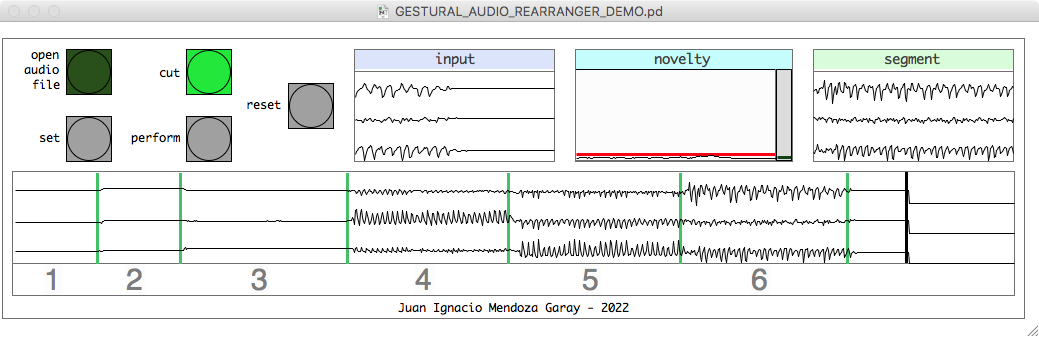
\includegraphics[trim={0.35cm 1.4cm 0.7cm 1.5cm}, clip=true, width=1\textwidth]{GUI_Cut_task}
\caption{Graphical user interface showing the Cut stage of the test task up to gesture 6 (see Figure~\ref{fig_6}). The bottom plot shows the triaxial acceleration signal over time, in which the green vertical lines indicate gesture boundaries. Notice that the peak of the novelty curve (plot up at the centre) corresponding to the last boundary is very small, barely touching the red threshold line (parameter $\theta$).}
%\vspace{0.5cm}
	\label{fig_5}
\end{figure*}

\begin{figure}[t!]
%\vspace{0.4cm}
	\centering
		\includegraphics[width=0.88\columnwidth]{gestures_task_explained}
	\caption{Segmentation task. Only the area enclosed in thicker lines was shown to participants. The descriptions were communicated verbally.}
	\label{fig_6}
%\vspace{0.5cm}
\end{figure}

\subsubsection{The Researcher}

Throughout  development of the system and until a functional version was completed, the researcher (i.e., author of this article) conducted iterative testing using an upbeat electronic dance music piece. This piece has a clear beat at a tempo of 128 BPM (beats per minute) and an energetic feel. The decision to use this kind of music was informed by previous research that has observed that electronic dance music stimulates bodily motion more than other music genres \cite{Burger_Toiviainen_2020}. These qualities were thought to be likely to prompt gestures that are repetitive and clear, which are useful qualities for the combination of accelerometer and segmentation algorithm to achieve good segmentation. 

At this point in the development, some gestures were found to work well with the system. Static gestures achieved by only changing the orientation of the ball are well segmented and recognised, and any combination of the six possible orthogonal orientations is robust. Since the ball shape is fully symmetrical, letters (A to F) were put on the orthogonal points to aid visually in manipulation (Figure~\ref{fig_2}, Right). Further gestures were found to work well, such as repetitive motion in any orthogonal direction. A sequence of gestures that was found to work well is shown in Figure~\ref{fig_6}. This sequence, its gestures and variations of them, work well with  parameters $n = 80$, $n_{min} = 28$, and $n_{filt} = 24$, at a sampling rate of 20 frames per second yielding $lag = 55$ frames (0.4 seconds, not including latency due to logical processing), and $\theta = 0.03$. For example, gesture 6 is a variation of 5 as it repeats the hit twice at each side. The first three gestures shown in Figure~\ref{fig_6} are very easy because the ball has only to be rotated. Gestures 4 to 6 involve repetitive motion and they might be more challenging to perform. In particular, the transition to one gesture to the next must be done fast enough so that the transition is not recognised as a gesture. As a further visual aid, a small arrow was placed on the ball next to the letters, indicating the direction of the next letter (Figure~\ref{fig_2}, Right).

Furthermore, extraction of features (e.g., zero-crossings, amplitude) from the triaxial accelerometry signal and from its magnitude vector, was implemented. They did not improve segmentation but,  because of being windowed processes, they did increase lag (i.e., frames needed for computation) and computation cost (i.e., logical processing). Therefore, development and testing continued using only raw acceleration, to demonstrate what is possible without using extracted features. 
	
When the system reached a functional point, other people were asked to be involved in the testing. This was done with the intention of evaluating the functionality of the system, meaning whether it works as the intended proof of concept, and to get feedback on the user experience. This evaluation was exploratory, as participants were allowed to discover new gestures that might work with the system and to freely express their opinions.

\subsubsection{Researchers and Students of Music}

Researchers and students of Musicology, Music Therapy and Music Education at the 
% \anonymize{fooooooooooooooooooooooo}
University of Jyväskylä
were invited to participate in group and individual sessions. Group sessions for students were arranged as part of lectures within the courses Music Technology and Embodied Music Cognition. In the first sessions the researcher explained the system by demonstrating the working gesture sequence (Figure~\ref{fig_6}). Then, the participants were invited to freely experiment with the system. However, understanding the operation logic often proved difficult, making the evaluation too slow. To make it faster, and to standardise the evaluations, in subsequent sessions participants were explicitly asked to perform the sequence. Also, they were shown a printed paper with only the enclosed rectangle shown in Figure~\ref{fig_6}. 

\begin{figure}[t!]
%\vspace{0.1cm}
	\centering
		\includegraphics[trim={0.2cm 0.2cm 0.8cm 0.5cm}, clip=true, width=1\columnwidth]{RN_experiment}
	\caption{Number of correctly segmented gestures by visitors at the outreach event. Only some participants tried the task a second time, shown in darker shade.}
	\label{fig_7}
\end{figure}

During these sessions a protocol was developed and settled as follows:

\textbf{1.}	The researcher demonstrates the task using the upbeat electronic dance music piece. The task comprises first the Cut stage and then the Perform stage, using the seven gestures shown in Figure~\ref{fig_6}. The sequence is displayed on a paper.

\textbf{2.}	The participant is invited to do the task. If in the Cut stage not all gestures were segmented successfully, the participant is invited to repeat the Cut. The participant is allowed to do this as many times as they want. Then, the participant is invited to try the Perform stage.

\textbf{3.}	The participant is invited to freely improvise and/or to use another piece of music. The other pieces of available music are a classical waltz performed by a chamber ensemble (54 BPM), a heavy metal song (80 BPM), and a grunge song (100 BPM). All these pieces have a binary metre (e.g., 4/4) except the waltz, having a ternary metre (e.g., 3/4). Also, a new-age piece is available, having no clear beat and therefore no perceivable metre. 

\textbf{4.}	If the participant has not already expressed their opinion on the experience, they are invited and encouraged to do so. At any time, the researcher shall write down observations such as number of gestures correctly segmented in a trial (step 2), comments and ideas expressed by and discussed with the participant, what piece of music is used, and if a new gesture is discovered.

\subsubsection{The General Public}

The task described in the previous subsection was incorporated to a presentation open to the general public in an outreach event at the 
% \anonymize{fooooooooooooooooooooooo}
University of Jyväskylä called “European Researcher’s Night”. 
The presentation ran for seven hours, and the following data was tabulated on a flip-chart: age, gender, number of gestures successfully segmented consecutively staring with the first, and observations (as in step 4 of the protocol described in the previous subsection).

Data of 23 participants was tabulated but qualitative data from more participants was recorded as explained further down this subsection. From the participants whose data was tabulated, all used the upbeat electronic dance music, except one. The data of the latter was discarded in order to assess only data corresponding the same music as stimulus. A total of 17 participants performed the task as intended. Of these participants, 10 were female, and 7 were male. Only six of them chose to perform the task for a second time, and in all these cases the second trial of the task improved (see Figure~\ref{fig_7}). The median of the first trials was 4 gestures, the median of the second trials was 6 and the median of the maxima was 5. No clear correlation between number of correct segments and age or gender was observed. Nonetheless, it was observed that most of the very young participants, less than 10 years old, had difficulty in understanding the task and therefore did not perform the gestures correctly. For this reason, data for most of the participants being less than 10 years old was not recorded. However, notes were taken, and the common observation was that while they would not do the task as intended, they could instead achieve correct segmentation by only changing the orientation of the ball, aided by the letters on it.

\subsubsection{Overall Assessment}

This subsection presents the overall observations made in the three testing phases described above. 

\textbf{Static gestures:} Any set of orientations that are different among them enough will work, but it was observed that the 6 orthogonal orientations along the 3 axes work flawlessly.

\textbf{Continuous gestures:} Any combination and variation of repeated movements along the 6 orthogonal orientations (or 3 orthogonal axes) will work well. These axes need not to be aligned with the horizon (i.e., they may be diagonal).  Movements that are sudden and energetic work best, as these have high acceleration and therefore are better measured by an accelerometer. The smoother the movement, the less acceleration it will produce and the less likely it will be detected by the system. However, other gestures that do not fully conform to this general description were spontaneously discovered by participants. One of them is the “baby rocking”, which consist in holding the ball with two hands and moving it describing an upwards concave curve. Variations of this motion were performed by other participants, by describing a partial circumference in other orientations. Also circular motions and ``8" figures were successfully detected, inasmuch as the speed, and therefore radial acceleration, was powerful enough to produce a novelty score above the set threshold ($\theta $).

\textbf{Transitions:} As explained at the beginning of subsection \ref{Testing}, meta-parameter $n_{min}$ sets a minimum duration for gestures to be detected. However, this parameter is fixed and if the transition from one gesture to the next is slow enough to have a duration equal or greater than $n_{min}$, the transition will be identified as a segment. If that segment is kept, in the Perform stage the system often will get stuck in it, due to the characteristics of the DTW algorithm (i.e., computation time is proportional to the length of the segment). This will result in a continuous repetition of a very short segment until and if a different gesture is recognised. However, interestingly, two participants mentioned that they liked the result. One of them referred to it as “a DJ effect”.

\textbf{Form factor:} Two participants of the second phase (researchers and students) suggested making the letters on the ball bigger, which was done for the outreach event (as seen in Figure 2). One of those participants also tried to use the device with closed eyes to explore the possibility of not having to look at the ball when manipulating it. This happened after the participant realised that it was necessary to look at the ball whenever changing its orientation and to look at the computer screen to see if the gesture was successfully segmented. A discussion ensued with this participant, which led to conclude that, since the ball is fully symmetric, it is not possible to be aware of its orientation without looking at it.

\textbf{User experience:} The task proved to be challenging to different extents. Some participants expressed that they wanted to try again to improve the number of correctly segmented gestures. All participants showed engagement and enjoyment. However, it is important to consider that participation was voluntary. It is to expect that researchers and students have interest as the experience is related to their profession and studies. Likewise, it may be safely assumed that visitors at the outreach event attended because they had curiosity about what they might be presented with.

\section{Discussion and Future Work}

The system described in this article is intended to be a proof of concept that demonstrates the feasibility of unsupervised learning of patterns in a continuous input signal, for gestural control, within a musical application. The unsupervised pattern learning is based on a segmentation process that ineluctably produces a lagged response. In other words, noticeable time passes between the occurrence of the change from one gesture to the next, and the reporting that it had occurred. Therefore, the system is not suitable to execute fast notes or rhythmic patterns. Nonetheless, the musical application presented in this article conforms to these constraints, further giving support to the concept of delayed control of musical sound.

The musical application allows a user to rearrange the playback of an audio file by performing distinct gestures with a hand-held device. The assessment reported in this article used audio files of recorded music and the meta-parameters of the system were adjusted for the experience with the chosen music. However, any audio recording may be used, and the parameters may be tweaked for further exploration that may lead to unexpected yet interesting results.

The assessment revealed that while the system is not able to segment all possible gestures, there is still a fairly rich variety of possible gestures, comprising static orientations and variations of dynamic gestures such as straight and curved trajectories in different orientations. This  result was obtained using a single setting of meta-parameters, showing a substantial degree of generalisation. This was unexpected, as the perceptual evaluation by 
% \anonymize{foooooooooooooooooo}
Mendoza \cite{Mendoza_2022}
suggested that fine-tuning might have been needed for each user. Furthermore, participants of the assessment tended to take the task as a challenge, which in combination with the discovery of new meaningful gestures, and the sense-making of the constraints, turned the experience into a ludic one.

While the assessment shows that the system is promising, also it prompted reflection on opportunities for improvement, firstly of the system presented here, and second, for the advancement of the concepts of delayed control and seamless human-machine musical interaction. Regarding the system presented in this article, one immediate improvement that could be made is the form factor. The hand-held device would improve by having a form that allows the user to manipulate it without needing to look at it. To that effect, the form needs to have rotational asymmetry, for example a ``boot'' shape as shown in Figure \ref{fig_8}.
	
\begin{figure}[t!]
	\centering
		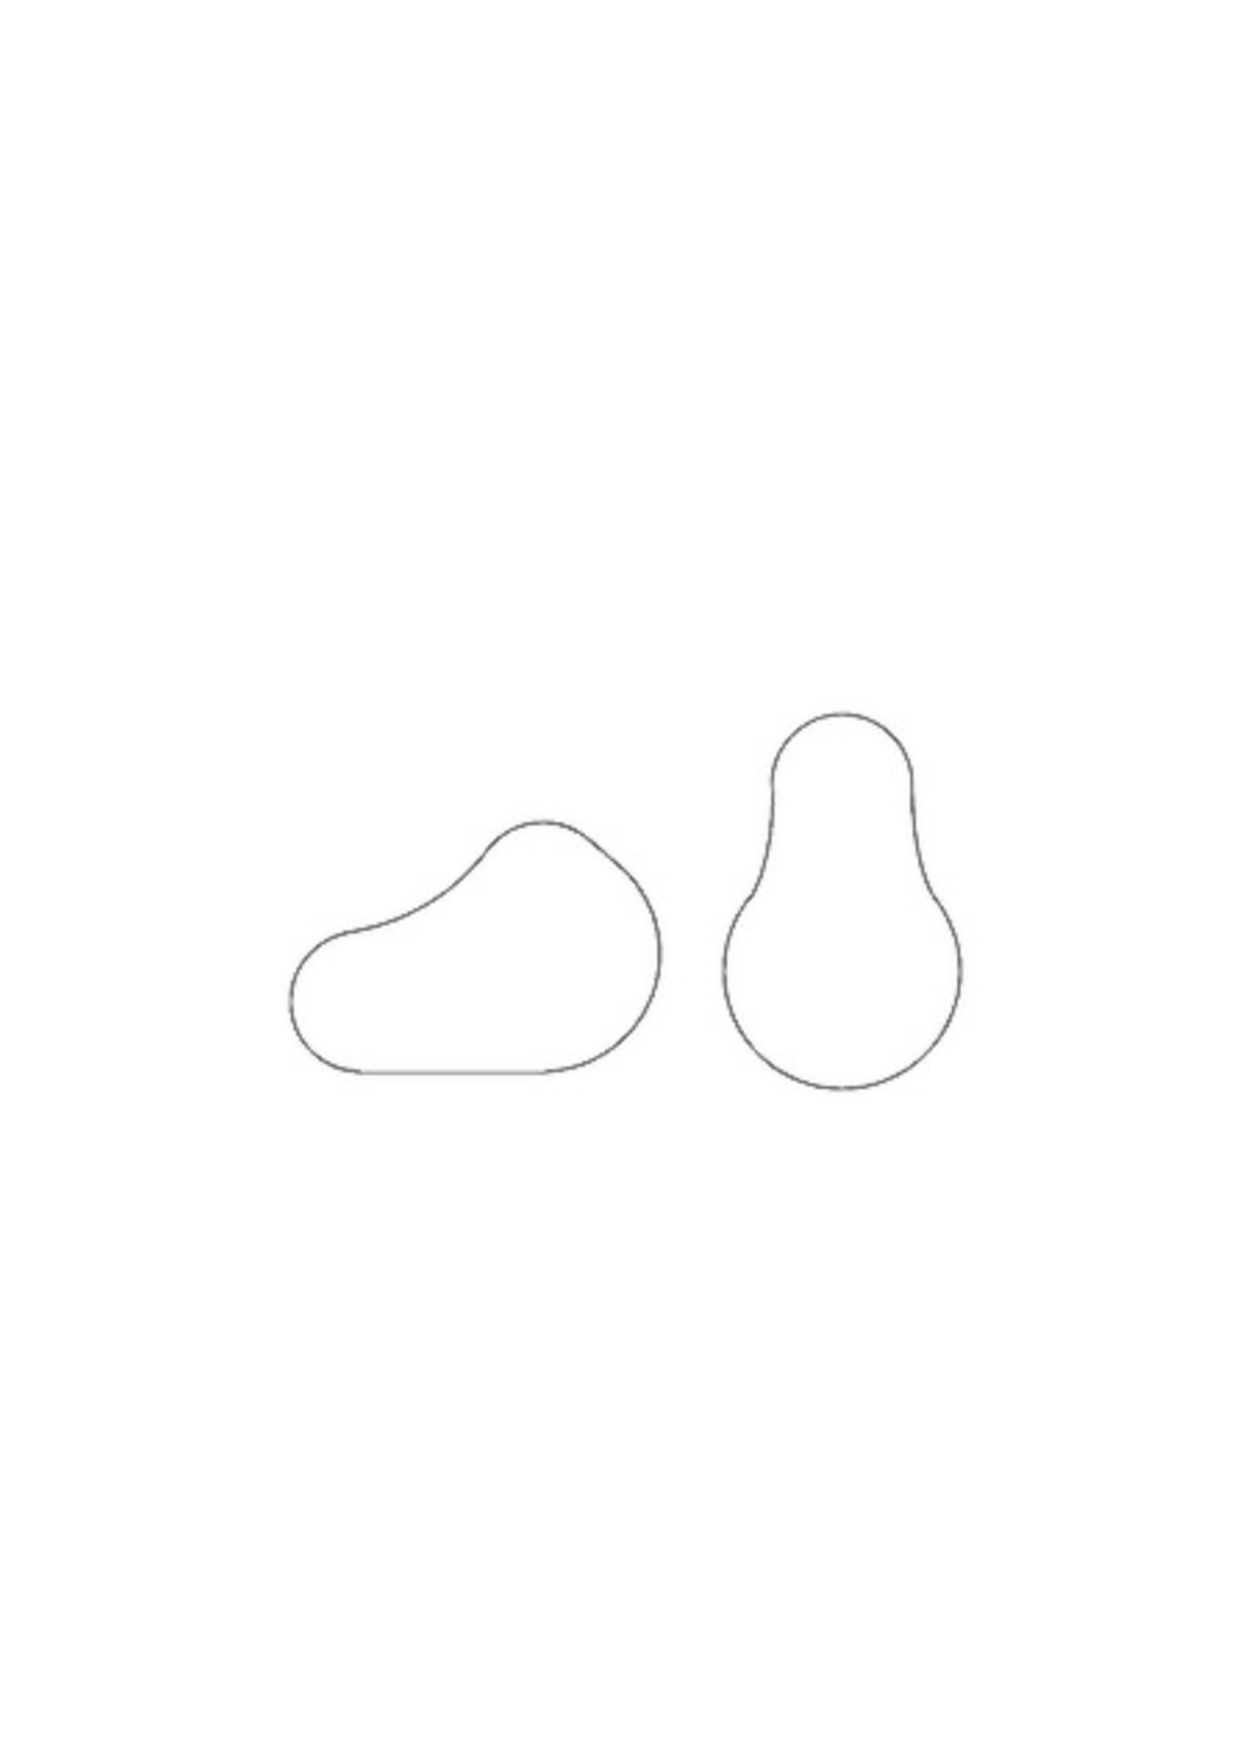
\includegraphics[trim={4cm 11.2cm 4cm 12cm}, clip=true, width=0.8\columnwidth]{boot_shape}
	\caption{Form having rotational asymmetry. Left -- lateral view. Right -- zenithal view.}
	\label{fig_8}
\end{figure}	 

Future research may consider the detection of patterns using features extracted from the triaxial acceleration signal. The features that may be extracted from the raw signal are several, for example zero-crossings or spectrum (i.e., computing a Fast-Fourier Transform). Also the magnitude (i.e., Euclidean norm) of the triaxial signal may be used to compute these or other features. Using these features will have an impact in the detection of novelty (and therefore the threshold parameter $\theta $) because of the information that the features carry. Additionally, the computation of features may have an impact on the overall latency of the system. 

Further variations of the system may include several sensors. For example, a second hand-held device may be incorporated, or sensors that are not hand-held but wearable, such as armbands or other contrivances to attach sensors to parts of the body. Other sensing technologies may be used as well, such as video tracking or skeleton recognition from video, or clothing that measures posture changes. The use of several sensors by more than one person at the same time would allow shared control, turning the experience into a group activity (e.g., \cite{Staudt_etal_2022, Tahiroglu_etal_2013}). Yet a further idea that may be explored in future research is the implementation of online multigranular segmentation, meaning the detection of gestural boundaries at different timescales (i.e., running parallel instances of the algorithm, each with a kernel of different width $n$). 

Current limitations to add more sensors, extracted features and the capability of multigranular segmentation, are algorithmic complexity, processing power and software efficiency. The two latter are due to the use of high-level programming and interconnected software, and the solution beyond using faster hardware is to implement the system using low-level programming. Arguably the best solution would involve the use of embedded software and hardware capable of parallel computing, such that the computing of different features and timescales is executed simultaneously. 

Moreover, it is important to consider that while the setting of meta-parameters generalised well given the specific configuration being tested in this study, a different setting might be needed when using other configurations of hardware, software, music and user. In this regard, it is convenient that future research considers scrutiny on the effects of the meta-parameters in the segmentation process and the user experience.

The online unsupervised temporal segmentation method described in this article has potential, as already insinuated, beyond the application described here. Consider that in the system presented here, the online segmentation procedure only contributes to display on the screen an indication when a gesture has been segmented in the Cut stage.  The display of a successfully detected gesture change-point occurs shortly after the actual change, depending on the set timescale. This allows the user, for example, to stop the Cut and restart if a gesture change was not detected. Arguably this is an advantage to the user, but presumably more can be done to exploit the online segmentation capability and thus it deserves more research to explore its further possibilities for near-real-time interaction. For example, a system may learn gestures as they occur. This may be incorporated to interactive systems where both the user and the system discover and learn gestures at the same time, leading to a seamless integration of human and machine with the purpose of making music.

%\end{document}  % This is where a 'short' article might terminate

\section{Ethical Standards}
All participants gave verbal informed consent for the use of their anonymous collected data, following the research ethics guidelines by the 
% \anonymize{fooooooooooooooooooooooo}
University of Jyväskylä.

%
% The following two commands are all you need in the
% initial runs of your .tex file to
% produce the bibliography for the citations in your paper.
\bibliographystyle{abbrv}

	\bibliography{delayed_control_unsupervised_segmentation} 

% You must have a proper ".bib" file
%  and remember to run:
% latex bibtex latex latex
% to resolve all references
%
% ACM needs 'a single self-contained file'!
%
%APPENDICES are optional
\appendix
Software and documentation: 
\href{https://gitlab.jyu.fi/juigmend/temporal_segmentation_gestural_control}{https://gitlab.jyu.fi/juigmend\\/temporal\_segmentation\_gestural\_control}
% \anonymize{fooooooooooooooooooooooo}

%%Appendix A
%\section{Headings in Appendices}
%The rules about hierarchical headings discussed above for
%the body of the article are different in the appendices.
%In the \textbf{appendix} environment, the command
%\textbf{section} is used to
%indicate the start of each Appendix, with alphabetic order
%designation (i.e. the first is A, the second B, etc.) and
%a title (if you include one).  So, if you need
%hierarchical structure
%\textit{within} an Appendix, start with \textbf{subsection} as the
%highest level. Here is an outline of the body of this
%document in Appendix-appropriate form:
%\subsection{Introduction}
%\subsection{The Body of the Paper}
%\subsubsection{Type Changes and  Special Characters}
%\subsubsection{Math Equations}
%\paragraph{Inline (In-text) Equations}
%\paragraph{Display Equations}
%\subsubsection{Citations}
%\subsubsection{Tables}
%\subsubsection{Figures}
%\subsubsection{Theorem-like Constructs}
%\subsubsection*{A Caveat for the \TeX\ Expert}
%\subsection{Conclusions}
%\subsection{Acknowledgments}
%\subsection{Additional Authors}
%This section is inserted by \LaTeX; you do not insert it.
%You just add the names and information in the
%\texttt{{\char'134}additionalauthors} command at the start
%of the document.
%\subsection{References}
%Generated by bibtex from your ~.bib file.  Run latex,
%then bibtex, then latex twice (to resolve references)
%to create the ~.bbl file.  Insert that ~.bbl file into
%the .tex source file and comment out
%the command \texttt{{\char'134}thebibliography}.
%
%
%% This next section command marks the start of
%% Appendix B, and does not continue the present hierarchy
%\section{More Help for the Hardy}
%The sig-alternate.cls file itself is chock-full of succinct
%and helpful comments.  If you consider yourself a moderately
%experienced to expert user of \LaTeX, you may find reading
%it useful but please remember not to change it.

%%% Place this command where you want to balance the columns on the last page. 
%\balancecolumns 

% That's all folks!
\end{document}
